\documentclass[letterpaper]{article}

\usepackage[margin=1in]{geometry}

\usepackage{graphicx}

\usepackage{array}

\usepackage{titlesec}
    \titlespacing*{\section}
        {0pt}{3ex}{0pt}

    \titlespacing*{\subsection}
        {0pt}{1.5ex}{1ex}

\setlength{\parindent}{0pt}

\newcommand{\horizontalLine}{%
    \rule{\textwidth}{0.2pt}
    \vspace{1ex}
}

\begin{document}
    \begin{tabular}{p{0.45\textwidth} >{\raggedleft\arraybackslash}m{0.45\textwidth}}
        {\Huge
        \textbf{Jason Ngo}}

        {\large
        Software Developer}
        &
        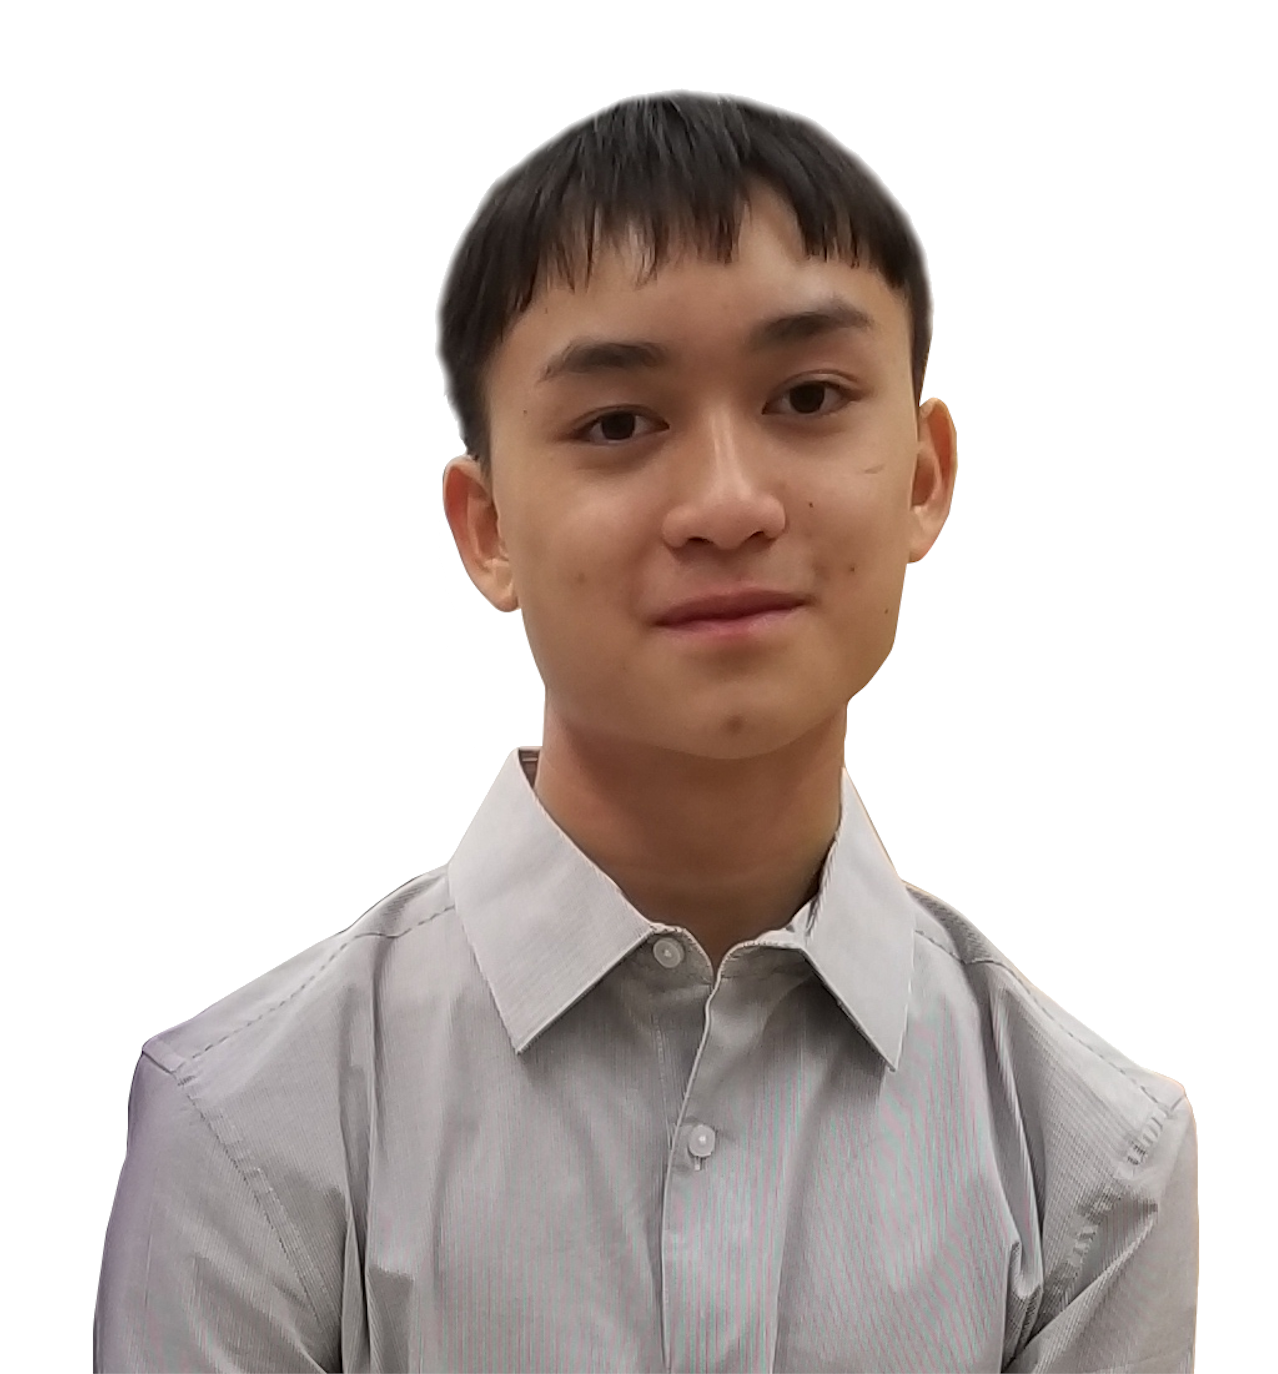
\includegraphics[width=0.15\textwidth]{../resources/pfp.png}
    \end{tabular}

    {\small%
        \renewcommand{\arraystretch}{1.5}
        \begin{tabular}{p{0.08\textwidth} p{0.2\textwidth} p{0.15\textwidth} p{0.45\textwidth}}
            \\
            \textbf{Address} & 3224 52 Ave NW & \textbf{GitHub} & github.com/Green-Avocado \\
            & Calgary, AB & \textbf{StackOverflow} & stackoverflow.com/users/13528169/green-avocado \\
            & T2L 1V5 & \textbf{LinkedIn} & linkedin.com/in/jasonn-dev \\
            \textbf{Mobile} & (587) 890-5250 & \textbf{Website} & jasonn.dev \\
            \textbf{Email} & work@jasonn.dev \\
            \\
        \end{tabular}
    }

    A current student looking to major in computer science.
    I have ongoing experience in software development as a freelancer.
    During my previous employment and volunteer experiences, I have consistently demonstrated my ability to work well in a team.
    Additionally, I am excellent with analytical thinking, problem solving, and communication.
    I am interested in further developing my existing skills as well as learning new technologies.

    \section*{Skills Summary}

        \rule{\textwidth}{0.2pt}

        \subsection*{Full-stack development}

        Proficient in the development of front-end and back-end solutions.
        Experience in creating intuitive and responsive user interfaces.
        Used a variety of technologies to create dynamic web content.

        \begin{center}
        \begin{tabular}{p{0.22\textwidth} p{0.22\textwidth} p{0.22\textwidth} p{0.22\textwidth}}
            HTML & CSS & Javascript & NodeJs \\
            PHP & Python & C++ & MySQL \\
            Firebase & Firestore & NGINX & Express \\
        \end{tabular}
        \end{center}

        \subsection*{Desktop development and scripting}

        Capable of developing programs ranging from simple scripts to larger applications.
        When possible, I tend to focus on creating well-structured, efficient programs.

        \begin{center}
        \begin{tabular}{p{0.22\textwidth} p{0.22\textwidth} p{0.22\textwidth} p{0.22\textwidth}}
            C & C++ & C\# & Python \\
            Bash &&&\\
        \end{tabular}
        \end{center}

        \subsection*{Technical writing}

        Able to use a variety of typesetting programs and word processors to produce detailed technical documentation.

        \begin{center}
        \begin{tabular}{p{0.22\textwidth} p{0.22\textwidth} p{0.22\textwidth} p{0.22\textwidth}}
            LaTeX & Microsoft Office & Libre Office & Google Drive \\
        \end{tabular}
        \end{center}

        \subsection*{Debugging and disassembly tools}
        Proficient with tools to effectively debug or disassemble programs compiled for x86 or x64 architecture.
        I have a good understanding of how memory is structured in both systems.

        \begin{center}
        \begin{tabular}{p{0.22\textwidth} p{0.22\textwidth} p{0.22\textwidth} p{0.22\textwidth}}
            GDB & Radare2 &&\\
        \end{tabular}
        \end{center}

        \subsection*{Version control}
        Ability to effectively use version control tools for managing projects, backups, and remotely collaborating with a team.
        I make use of and contribute to open source projects through GitHub.

        \begin{center}
        \begin{tabular}{p{0.22\textwidth} p{0.22\textwidth} p{0.22\textwidth} p{0.22\textwidth}}
            Git & Subversion &&\\
        \end{tabular}
        \end{center}

        \subsection*{Linux}

        Years of personal experience using different distributions of Linux.
        Very familiar with the use of the command line and Bash.
        Experience in operating a Linux server.

        \begin{center}
        \begin{tabular}{p{0.22\textwidth} p{0.22\textwidth} p{0.22\textwidth} p{0.22\textwidth}}
            Debian and derivatives & Arch and derivatives &&\\
        \end{tabular}
        \end{center}

        \subsection*{Text editors, compilers, and IDEs}
        Well versed in a variety of tools for writing and compiling programs.
        I am familiar with the different workflows involved in the use of each of these programs.

        \begin{center}
        \begin{tabular}{p{0.22\textwidth} p{0.22\textwidth} p{0.22\textwidth} p{0.22\textwidth}}
            Visual Studio & Notepad++ & Vim & Atom \\
            GCC & G++ & Makefile & CMake \\
        \end{tabular}
        \end{center}

    \section*{Work Experience}

        \horizontalLine

        \begin{tabular}{p{0.2\textwidth} p{0.7\textwidth}} 
            \textbf{2020/04 - Present} & \large\textbf{Freelance Software Developer} \\
            & Worked individually or in a small team to develop desktop applications and web applications according to client specifications. \\
            \\
            \textbf{2016/06} & \large\textbf{Calgary Stampede Work Experience Program} \\
            & \emph{Boys and Girls Clubs of Calgary, Calgary, AB} \\
            & Worked in a team of six under supervision to patrol a designated area during the Calgary Stampede event and ensure that the area remained presentable. \\
        \end{tabular}

    \section*{Education}

        \horizontalLine

        \begin{tabular}{p{0.2\textwidth} p{0.7\textwidth}} 
            \textbf{2020/09 - 2024/04} & \large\textbf{Bachelor of Science} \\
            (Anticipated) & \emph{University of British Columbia, Vancouver, BC} \\
            \\
            \textbf{2017/09 - 2020/06} & \large\textbf{Alberta High School Diploma} \\
            & \emph{Sir Winston Churchill High School, Calgary, AB} \\
            \\
            \textbf{2018/02 - 2020/05} & \large\textbf{International Baccalaureate Diploma Programme} \\
            & \emph{Sir Winston Churchill High School, Calgary, AB} \\
        \end{tabular}

    \section*{Volunteering}

        \horizontalLine

        \begin{tabular}{p{0.2\textwidth} p{0.7\textwidth}} 
            \textbf{2018/02 - 2020/02} & \large\textbf{Volunteer Churchill} \\
            & \emph{Sir Winston Churchill High School, Calgary, AB} \\
            & Participated in a variety of community-oriented projects as a volunteer. \\
            \\
            \textbf{2015/07 - 2019/07} & \large\textbf{Pool Assistant/Program Assistant} \\
            & \emph{Village Square Leisure Centre, Calgary, AB} \\
            & Assisted in running day camp programs and swimming lessons as a volunteer.
            Worked directly with project leaders, supervisors, and other volunteers. \\
        \end{tabular}

    \section*{Activities}

        \horizontalLine

        \begin{tabular}{p{0.2\textwidth} p{0.7\textwidth}} 
            \textbf{2019/09 - Present} & \large\textbf{CTF Events} \\
            & \emph{https://ctftime.org/} \\
            & Wrote scripts to automate interactions with a server to solve challenges under time constraints.
            Reverse engineered programs through source code or disassembled binaries without symbols.
            Identified and exploited security vulnerabilities in web applications and disassembled binaries. \\
            \\
            \textbf{2017/09 - 2020/02} & \large\textbf{Vex Robotics Club} \\
            & \emph{Sir Winston Churchill High School, Calgary, AB} \\
            & Wrote programs which interacted with the Vex API to receive user input and relay instructions to motors.
            Designed programs for storing and implementing predefined autonomous movements, and wrote scripts to facilitate modification of autonomous program files. \\
        \end{tabular}

    \section*{Awards}

        \horizontalLine

        \begin{tabular}{p{0.2\textwidth} p{0.7\textwidth}} 
            \textbf{2020/03} & \large\textbf{Vex Alberta Provincial Tournament - Think Award} \\
            & \emph{4414 Crowchild Trail SW, Calgary, AB} \\
            & Awarded for innovative, well written code.
            I was the lead programmer for our robot and was instrumental in achieving this award. \\
            \\
            \textbf{2019/04} & \large\textbf{Science Engineering and Technology Challenge} \\
            & \emph{University of Calgary, Calgary, AB} \\
            & Achieved first place in a multi-disciplinary event.
            Worked closely with a small team, competing against teams from highschools across Canada. \\
            \\
        \end{tabular}

    \section*{Projects}

        \horizontalLine

        \begin{tabular}{p{0.2\textwidth} p{0.7\textwidth}} 
            \textbf{2020/06 - Present} & \large\textbf{Personal Web Server} \\
            & \emph{https://github.com/Green-Avocado/nodejs-personal-web-server.git} \\
            & Simple webserver running NGINX and NodeJs on Arch Linux. \\
            \\
            \textbf{2020/06 - Present} & \large\textbf{CTF Writeups} \\
            & \emph{https://github.com/Green-Avocado/CTF.git} \\
            & Documentation of attempts at CTF challenges and in-depth explanations of solutions. \\
            \\
            \textbf{2020/05 - 2020/06} & \large\textbf{Resumes and CV} \\
            & \emph{https://github.com/Green-Avocado/Resume.git} \\
            & LaTeX source code for my resumes and my CV. \\
            \\
            \textbf{2020/05 - 2020/06} & \large\textbf{COVIDPing Image Generator} \\
            & \emph{https://github.com/Green-Avocado/covidping-image-generation.git} \\
            & Web application for generating and displaying Twitter cards for COVID-19 statistics in US states. \\
        \end{tabular}

\end{document}

